\documentclass[12pt]{report}

% ==== Paquetes ====
\usepackage[utf8]{inputenc}
\usepackage[T1]{fontenc}
\usepackage[spanish]{babel}
\usepackage{amsmath, amssymb}
\usepackage{graphicx}
\usepackage{hyperref}
\usepackage{geometry}
\usepackage{hyperref}[hidelinks]
\geometry{a4paper, margin=2.5cm}

% ==== Datos del informe ====
\title{Manual de instalación para el uso del USRP 2920}
\author{Equipo de trabajo - Miercoles 9am - 11am \\ Universidad Nacional San Antonio Abad del Cusco \\ Davis Bremdow Salazar Roa - 200353}
\date{\today}

\begin{document}
	
	% Portada
	\maketitle
	
	% ==== Capítulo 1 ====
	\chapter{Instalación}
	
	\section{Introducción}
	El dispositivo de Radio Definido por Sofware USRP 2920 es un transceptor RF modificable mediante software que permite procesar señales de información mediante un programa definido con un entorno mediante labview, GNU Radio (Radioconda) o Matlab, sin embargo para hacer uso de estos entornos es necesaria la instalación de un driver o controlador que permite realizar la interacción entre el dispositivo físico y el software de preferencia.
	
	Para este caso debido a la extensa documentación y ejemplos en línea se explicará la conexión entre el USRP y GNU Radio.
	
	\section{Instaladores}
	Para realizar esta conexión es necesario realizar la descargar de los drivers para:
	\begin{itemize}
		\item Drivers - USRP 2920 - \href{https://files.ettus.com/binaries/uhd/latest_stable/4.8.0.0/}{Descarga}
		\item GNU Radio - \href{https://github.com/gnuradio/gnuradio/releases}{Descarga}
	\end{itemize}
	

	
	\section{Configuración del puerto Ethernet}
	Una vez instalados ambos programas se puede proseguir con la conexión entre el USRP y la computadora mediante el puerto Ethernet, siendo necesario además configurar este puerto con una dirección IP estática de la forma \textbf{192.168.10.x} donde \textbf{x} es la dirección diferente a la definida por el USRP.
	\newpage
	
	Para esta configuración es necesario acceder a las propiedades del puerto ethernet y seleccionar la último opción vista en la imagen \ref{fig:conexion-ethernet}.
	
	\begin{figure}[h]
		\centering
		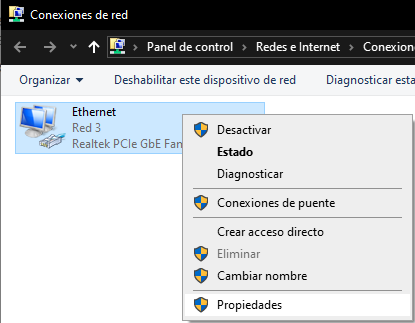
\includegraphics[width=0.4\linewidth]{media/conexion-ethernet}
		\caption{Configuración del puerto Ethernet - I}
		\label{fig:conexion-ethernet}
	\end{figure}
	
	Seguidamente se debe elegir la configuración del \textbf{Protocolo de Internet versión 4}
	
	\begin{figure}[h]
		\centering
		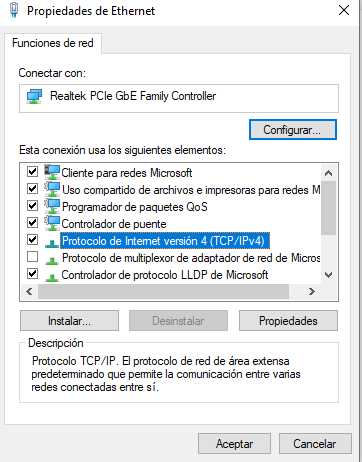
\includegraphics[width=0.4\linewidth]{media/conexion-ethernet2}
		\caption{Configuración puerto Ethernet - II}
		\label{fig:conexion-ethernet2}
	\end{figure}
	
	\newpage
	Y finalmente en la interfaz se debe configurar la siguiente dirección IP la cual se elige para evitar un conflicto con el USRP 2920 que tienen asignados las direcciones \textbf{192.168.10.2} y \textbf{192.168.10.3} respectivamente para cada dispositivo.
	
	\begin{figure}[h]
		\centering
		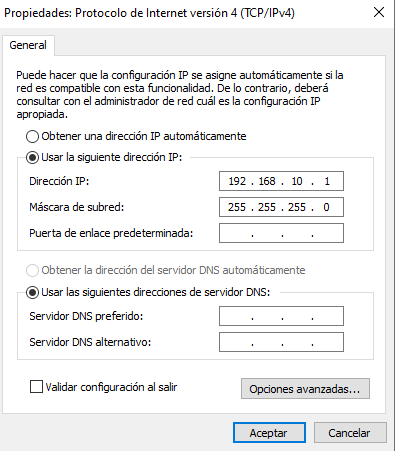
\includegraphics[width=0.5\linewidth]{media/conexion-ethernet3}
		\caption{Configuración Puerto Ethernet - III}
		\label{fig:conexion-ethernet3}
	\end{figure}
	
	\chapter{GNU Radio}
	
	\section{Configuración de bloques}
	En la interfaz de GNU Radio se deben buscar los bloques
	
	\begin{itemize}
		\item UHD: USRP Source
		\item QT GUI Sink
	\end{itemize}
	
	Y se debe realizar el conexionado como se muestra en la figura \ref{fig:gnu-radio-bloques} 
	
	\begin{figure}[h]
		\centering
		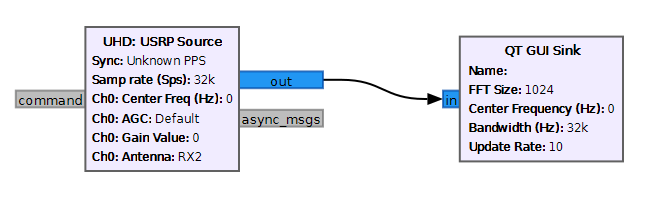
\includegraphics[width=0.6\linewidth]{media/gnu-radio-bloques}
		\caption{Configuración de bloques en GNU - Radio}
		\label{fig:gnu-radio-bloques}
	\end{figure}
	
	Ello con la finalidad de poder verificar la conexión entre  el USRP y GNU Radio, siendo una \textbf{ejecución exitosa} en caso se tenga la visualización de una ventana gráfica perteneciente al bloque \textbf{QT GUI Sink}.
	
	\newpage
	Finalmente se debe tener en consideración la configuración del bloque \textbf{UHD: USRP Source} en la cual el campo \textbf{Device Address} y el campo \textbf{Sync} deben tener la configuración mostrada en la figura \ref{fig:gnu-radio-bloques-source}
	
	\begin{figure}[h]
		\centering
		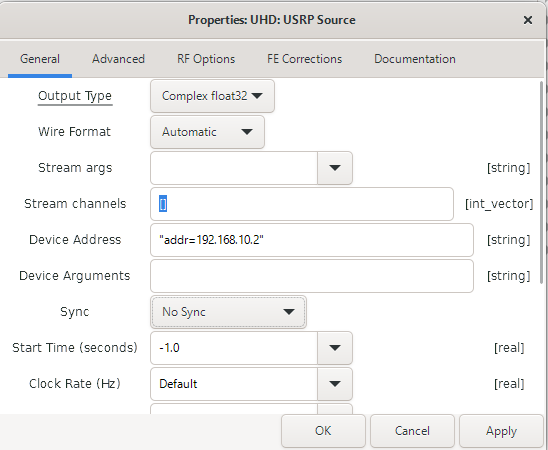
\includegraphics[width=0.6\linewidth]{media/gnu-radio-bloques-source}
		\caption{Configuración del bloque UHD Source}
		\label{fig:gnu-radio-bloques-source}
	\end{figure}
	
	En donde el campo \textbf{Device Address} tendrá una ligera variación según el USRP a utilizar y su configuración.
	
	% ==== Bibliografía ====
	%\bibliographystyle{plain}   % o "ieeetr", "apalike", etc.
	%\bibliography{referencias}  % Sin extensión .bib
	
\end{document}
